\chapter{Law of Large Numbers}
\section{Convergence in Probability}

\vspace{1em}

\begin{definitionbox}{Convergence in Probability}
The sequence of random variables \( X_1, X_2, X_3, \ldots, X_n, \ldots \) is said to \textbf{converge in probability} to the constant \( c \), if for every \( \epsilon > 0 \),
\[
\lim_{n \to \infty} P\left( |X_n - c| \leq \epsilon \right) = 1
\]
or equivalently,
\[
\lim_{n \to \infty} P\left( |X_n - c| > \epsilon \right) = 0
\]

\noindent \textbf{Notation:} \( X_n \xrightarrow{P} c \)
\end{definitionbox}

\vspace{1em}

This concept plays a key role in the Law of Large Numbers, where the sample mean of independent and identically distributed random variables converges in probability to the population mean as the sample size grows.

\vspace{2em}

\begin{definitionbox}{Chebyshev’s Inequality}
Let \( X \) be a random variable with finite mean \( \mu \) and variance \( \sigma^2 \). Then, for any \( k > 0 \),
\[
P\left( |X - \mu| \geq k \right) \leq \frac{\sigma^2}{k^2}
\]

\textit{Using complements:}
\[
P\left( |X - \mu| < k \right) \geq 1 - \frac{\sigma^2}{k^2}
\]
\end{definitionbox}

\newpage

\vspace*{1em}

\begin{definitionbox}{Weak Law of Large Numbers (WLLN)}
Let \( X_1, X_2, \ldots \) be a sequence of independent and identically distributed random variables, each having finite mean \( E(X_i) = \mu \) and variance \( \mathrm{Var}(X_i) = \sigma^2 \). Then, for any \( \epsilon > 0 \),
\[
P\left( \left| \frac{X_1 + X_2 + \cdots + X_n}{n} - \mu \right| \geq \epsilon \right) \to 0 \quad \text{as } n \to \infty
\]

\noindent\textbf{Notation:} \( \bar{X}_n \xrightarrow{P} \mu \)
\end{definitionbox}
\subsection*{Proof of the Weak Law of Large Numbers (WLLN)}

We aim to show that for every \( \epsilon > 0 \),
\[
\lim_{n \to \infty} P\left( \left| \bar{X}_n - \mu \right| > \epsilon \right) = 0
\]
where \( \bar{X}_n \) is the sample mean of \( n \) independent and identically distributed (i.i.d.) random variables with
\[
E(X_i) = \mu, \quad \text{and} \quad \mathrm{Var}(X_i) = \sigma^2.
\]

Let
\[
\bar{X}_n = \frac{1}{n} \sum_{i=1}^{n} X_i.
\]

By the Central Limit Theorem (CLT), we know that
\[
\bar{X}_n \sim \mathcal{N} \left( \mu, \frac{\sigma^2}{n} \right).
\]

Now, applying \textbf{Chebyshev’s Inequality}, which states that for any random variable \( X \) with mean \( \mu \) and variance \( \sigma^2 \),
\[
P\left( |X - \mu| > k \right) \leq \frac{\sigma^2}{k^2} \quad \text{for } k > 0,
\]
to \( \bar{X}_n \), we set \( k = \epsilon \), and obtain:
\[
P\left( \left| \bar{X}_n - \mu \right| > \epsilon \right) \leq \frac{\mathrm{Var}(\bar{X}_n)}{\epsilon^2} = \frac{\sigma^2 / n}{\epsilon^2} = \frac{\sigma^2}{n \epsilon^2}.
\]

Taking the limit as \( n \to \infty \), we have:
\[
\lim_{n \to \infty} P\left( \left| \bar{X}_n - \mu \right| > \epsilon \right) \leq \lim_{n \to \infty} \frac{\sigma^2}{n \epsilon^2} = 0.
\]

Since probabilities are always non-negative, we conclude:
\[
\lim_{n \to \infty} P\left( \left| \bar{X}_n - \mu \right| > \epsilon \right) = 0.
\]

By the definition of convergence in probability,
\[
\bar{X}_n \xrightarrow{P} \mu.
\]
\qed
\section*{Example: Poisson Convergence via WLLN}

Let \( X_i \), for \( i = 1, 2, 3, \ldots \), be independent Poisson random variables with rate parameter \( \lambda = 3 \). Prove that:
\[
\bar{X}_n \xrightarrow{P} 3
\]

\textbf{Properties of Poisson Distribution:}
\[
E(X_i) = \lambda, \quad \mathrm{Var}(X_i) = \lambda
\]
In this case, \( \lambda = 3 \), so:
\[
E(X_i) = \mathrm{Var}(X_i) = 3
\]

\textbf{Proof:}

We know:
\[
E\left( \frac{X_1 + X_2 + \cdots + X_n}{n} \right) = 3, \quad \text{and} \quad
\mathrm{Var}\left( \frac{X_1 + X_2 + \cdots + X_n}{n} \right) = \frac{3}{n}
\]

Applying Chebyshev’s Inequality:
\[
P\left( \left| \frac{X_1 + X_2 + \cdots + X_n}{n} - 3 \right| \geq \epsilon \right) \leq \frac{3}{n \epsilon^2}
\]

Taking the limit as \( n \to \infty \):
\[
P\left( \left| \frac{X_1 + X_2 + \cdots + X_n}{n} - 3 \right| \geq \epsilon \right) \to 0
\]

\textbf{Conclusion:}
\[
\bar{X}_n \xrightarrow{P} 3
\]

\begin{figure}[h!]
  \centering
  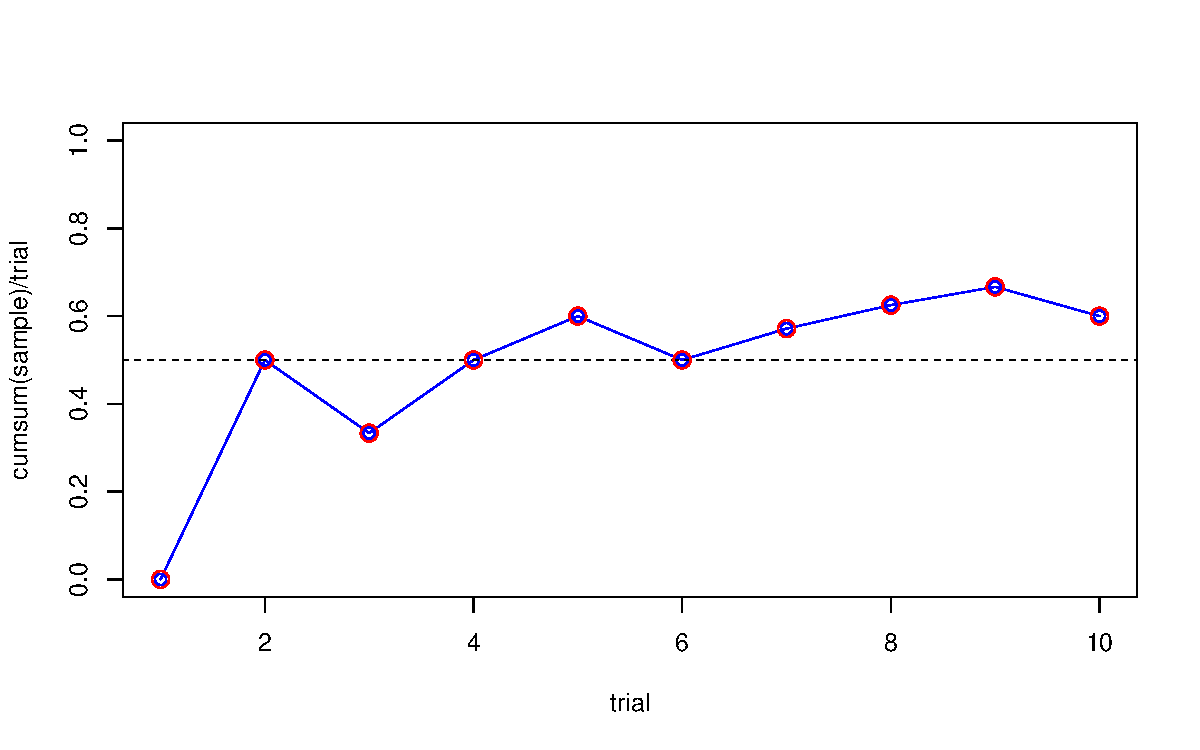
\includegraphics[width=0.72\textwidth]{Section5/simulation_plot.pdf}
  \caption{Simulation of running sample mean of Bernoulli(\(p = 0.5\)) trials over time.}
\end{figure}

{\color{gray} \textbf{R Simulation Code (Single Sample Path)}}

\begin{verbatim}
n = 10
trial = seq(1, n, by = 1)
sample = rbinom(n, 1, 1/2)

plot(trial, cumsum(sample)/trial, type = "l", ylim = c(0,1), col = "blue")
points(trial, cumsum(sample)/trial, col = "red")
abline(h = 0.5, lty = 2, col = "black")
\end{verbatim}

\begin{figure}[h!]
  \centering
  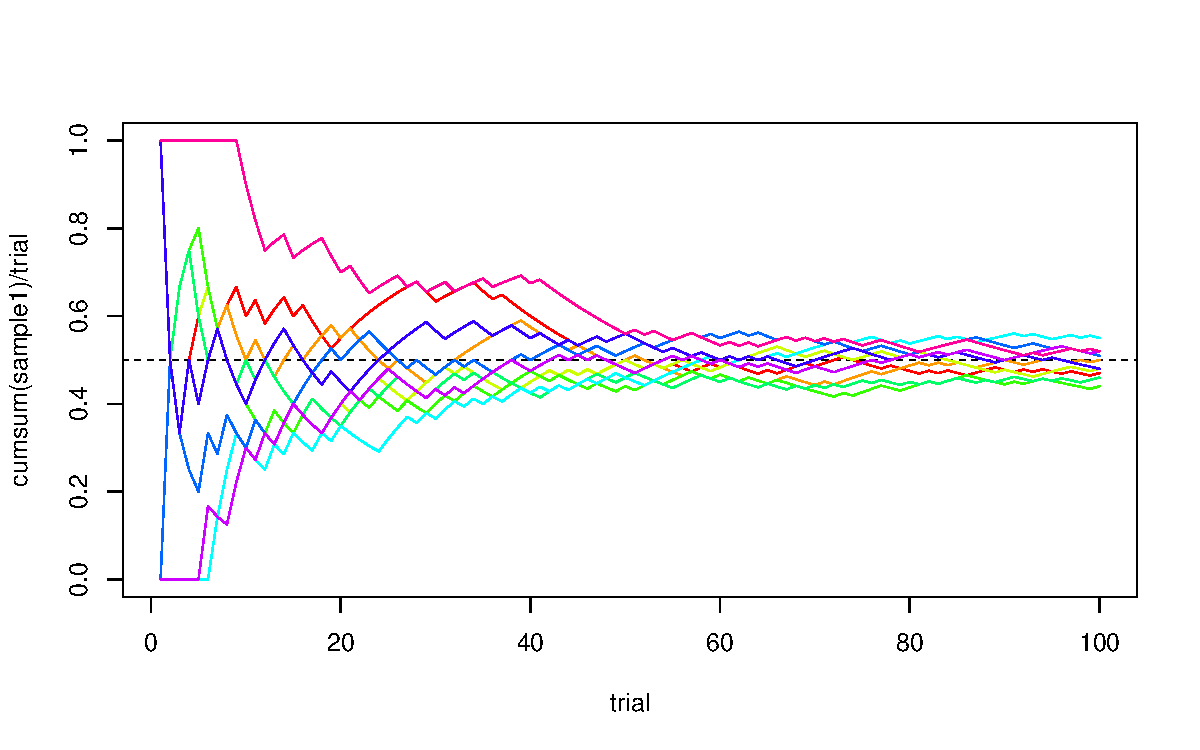
\includegraphics[width=0.72\textwidth]{Section5/simulation_multi.pdf}
  \caption{Simulation of 10 running sample means of Bernoulli(\(p = 0.5\)) trials converging over 100 trials.}
\end{figure}


{\color{gray} \textbf{R Simulation Code (Multiple Sample Paths)}}


\begin{verbatim}
n = 100
trial = seq(1, 100, by = 1)

sample1 = rbinom(n, 1, 1/2)
sample2 = rbinom(n, 1, 1/2)
sample3 = rbinom(n, 1, 1/2)
sample4 = rbinom(n, 1, 1/2)
sample5 = rbinom(n, 1, 1/2)
sample6 = rbinom(n, 1, 1/2)
sample7 = rbinom(n, 1, 1/2)
sample8 = rbinom(n, 1, 1/2)

colors = rainbow(8)


plot(trial, cumsum(sample1)/trial, type = "l", col = colors[1], ylim = c(0,1))
lines(trial, cumsum(sample2)/trial, col = colors[2])
lines(trial, cumsum(sample3)/trial, col = colors[3])
lines(trial, cumsum(sample4)/trial, col = colors[4])
lines(trial, cumsum(sample5)/trial, col = colors[5])
lines(trial, cumsum(sample6)/trial, col = colors[6])
lines(trial, cumsum(sample7)/trial, col = colors[7])
lines(trial, cumsum(sample8)/trial, col = colors[8])
abline(h = 0.5, lty = 2, col = "black")
\end{verbatim}


\subsection*{Empirical Probability Insight}


The Law of Large Numbers gives us empirical probabilities. Consider tossing a fair coin. Define the random variable \( X \) as:

\[
X = \begin{cases}
1 & \text{heads up} \\
0 & \text{tails up}
\end{cases}
\]

Then as we sample more and more values of \( X \), the sample mean \( \bar{X}_n \) converges in probability to \( P(\text{heads up}) \), that is:

\[
\bar{X}_n \xrightarrow{P} P(\text{heads up}) 
\]


